%\subsection{Elektromyografi}
%EMG er en målemetode, som måler elektrisk aktivitet genereret af musklerne \citep{chowdhury2013}. 
%En EMG-måling dækker over et samlet antal potentialer fra måleområdet, idet der aktiveres mange muskelfibre \citep{keenan2012}. \fxnote{Ved ikke, om der skal skrives noget om, at muskelfiberne inaverers af motorneuroner, og at mængden af muskelfibre pr. motorneuron afhænger af musklen og dens funktion = det ville være godt, inddrag lidt ALS - KOMMENTAR: lige nu syntes vi ikke at der er relevant}

%Der kan anvendes to forskellige typer af EMG-målinger. Den ene er en ikke-invasiv metode, der kaldes overflade-EMG, og den anden er en invasiv metode, intramuskulær EMG \citep{chowdhury2013, keenan2012}. Hertil anvendes sidstnævnte i dette projekt. 
%Ved generel anvendelse af EMG-målinger, benyttes frekvensområdet ved $10-500~Hz$, hvorfor signaler uden for dette frekvensområde kan betegnes som støj \citep{morre2003, keenan2012}.  

%Denne metode kan påvirkes af flere artefakter, som bevægelsespåvirkning og støjpåvirkning fra elnettet ($50~Hz$) \citep{keenan2012}.
%Ligeledes kan der ved EMG-målinger fremkomme elektrisk støjpåvirkning fra omkringliggende muskler i forhold til området, der måles på. Dette betegnes som crosstalk \citep{keenan2012}. 

\subsection{Elektromyografi}
Til behandling af EMG-signalet, anvendes Muscle Sensor V3, der fremover refereres som 'EMG-forstærker'. Denne komponent måler en differens af de elektriske potentialer der måles gennem elektroderne. EMG-forstærkeren overholder de opstillede krav, og kan anvendes direkte med mikrokontrolleren. EMG-forstærkeren består af en intrumenteringsforstærker, et passivt højpasfilter, en full-wave rectifier, et aktivt lavpass filter og en justerbar forstærker \citep{advancertech2013}. 

En illustration af, hvordan EMG-forstærkeren behandler et inputsignal fremgår af \autoref{fig:sinussignal}.
\begin{figure}[H]
\centering
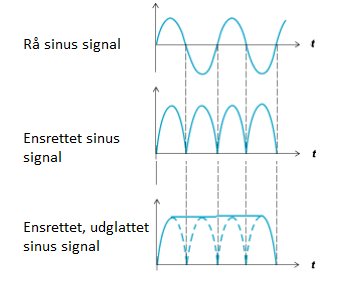
\includegraphics[width=0.6\textwidth]{figures/sinussignal.png}
\caption{Tre sinussignaler. Henholdsvis et råt, ensrettet og ensrettet samt udglattet. \citep{advancertech2013}.}
\label{fig:sinussignal}
\end{figure}

Med udgangspunkt i \autoref{fig:sinussignal} ses signalet som sinuskurven. Hertil passerer det højpasfilteret der dæmper DC støjen og dermed offsettet i signalet. Dette ses som signalet sinuskurven der svinger omkring 0, og er nødvendig for at ensretningen viker efter hensigten. Dernæst ensrettes signalet, således de negative værdier inverteres, og at der kun er svingninger i positiv retning. Herefter fortages et envalope, hvilket ses som det udglattede signal, hvortil der er beregnet en knækfrekvens på $1,94~Hz$, ud fra \autoref{eq:lavcutfre}. 

\begin{equation}\label{eq:lavcutfre}
f_c = \frac{1}{2 \pi C R} = \frac{1}{2 \pi \dot 1 \dot 10^{-6}F \dot 80,6 \dot 10^3\Omega} = 1,94~Hz
\end{equation}

EMG-forstærkeren har en minimum spændingsforsyning på $\pm 3~V$ samt en maksimal spændingsforsyning på $\pm 30~V$. Herudover er der mulighed for at justere gain med en faktor fra 0,002 til 20,700. \citep{advancertech2013}. 





%Synes ikke det passer ind her? Er det ikke meningen dette skal være mere overordnet, og så specificerer vi os senere til hvordan vi vil måle, sådan til vores forsøg?
%Den ene elektrode placeres over enten rectus femoris eller vastus intermedius (sidder under rectus femoris) og den anden elektrode placeres over biceps femoris. Reference elektroden placeres ved??.. 


%Støj kan reduceres ved at placere en 0.1 mikro f capacitor i nærheden, det er dog nødvendigt at tilføje mere, hvis der er 50 KHz støj, da det vil kunne resultere i fejl i accelerations målingen. Støjens tæthed vil forminskes i takt med at forsyningsspændingen forøges.
%Fase sensitiv demodulation teknikker er anvendt for at bestemme magnituden samt accelerationens retning. Demodulator outputtet er forstærket og bragt igennem en 32 k ohm modstand. – noget med det forebygger aliasing 
%  - Jeg ser dette som 'ligegyldigt' nu, da det handler om kondensator og støj. Kan ikke se hvorfor det skal bruges (endnu) måske skal det bruges efter vi har lavet pilotforsøg, hvis der viser sig meget støj





